\chapter{ویژگی از دید کاربر}

\section{کلاینت}
همانطور که اشاره کردیم کلاینت این پروژه از Next.js استفاده می‌کند.
طراحی رابط کاربری در محیط Figma انجام شده است.


مراحل پیاده سازی به شرح زیر است:
\begin{enumerate}
    \item دیزاین توکن ها را استخراج و به پروژه اضافه می‌کنیم. مانند رنگ ها، فاصله ها و سایه ها
    \item المنت های دیزاین سیستم رو پیاده سازی می‌کنیم. کامپوننت هایی مانند دکمه، اینپوت و کانتینر
    \item با کنار هم قرار دادن المنت های دیزاین سیستم و کامپونتت های مخصوص هر بخش، صفحه را تکمیل می‌کنیم
    \item مراحل دریافت یا فرستان اطلاعات را انجام می‌دهیم
    \item مرحله ۳ و ۴ را برای هر صفحه تکرار میکنیم
\end{enumerate}

\newpage

\begin{figure}[htbp]
    \centering
    \begin{subfigure}[b]{0.26\textwidth}
        \centering
        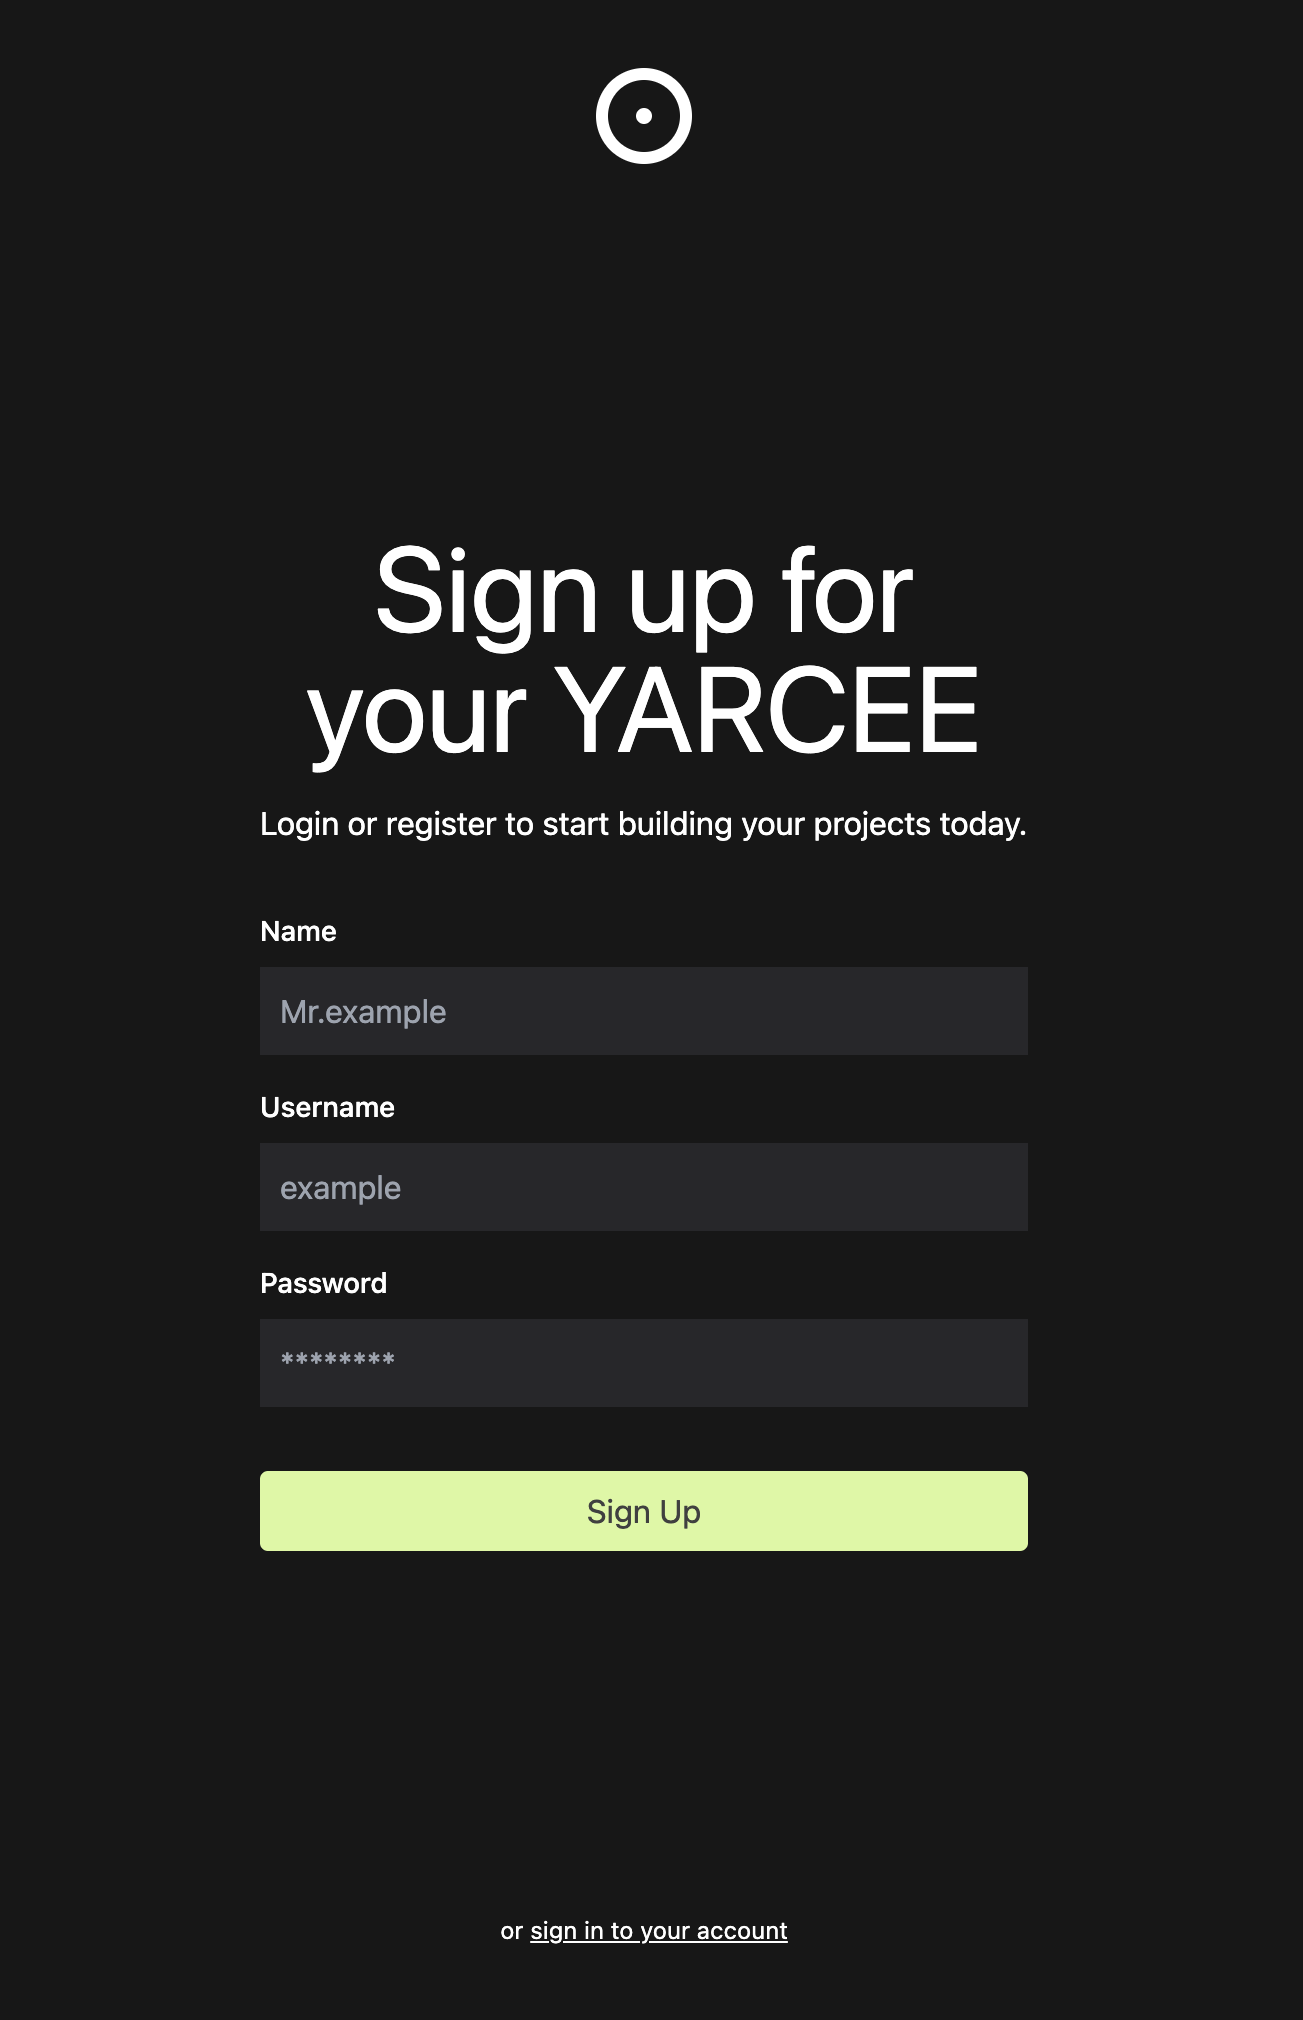
\includegraphics[width=\textwidth]{./3-Design/signup.png}
        \caption{صفحه ثبت نام}
        \label{fig:signup}
    \end{subfigure}
    \hfill
    \begin{subfigure}[b]{0.70\textwidth}
        \centering
        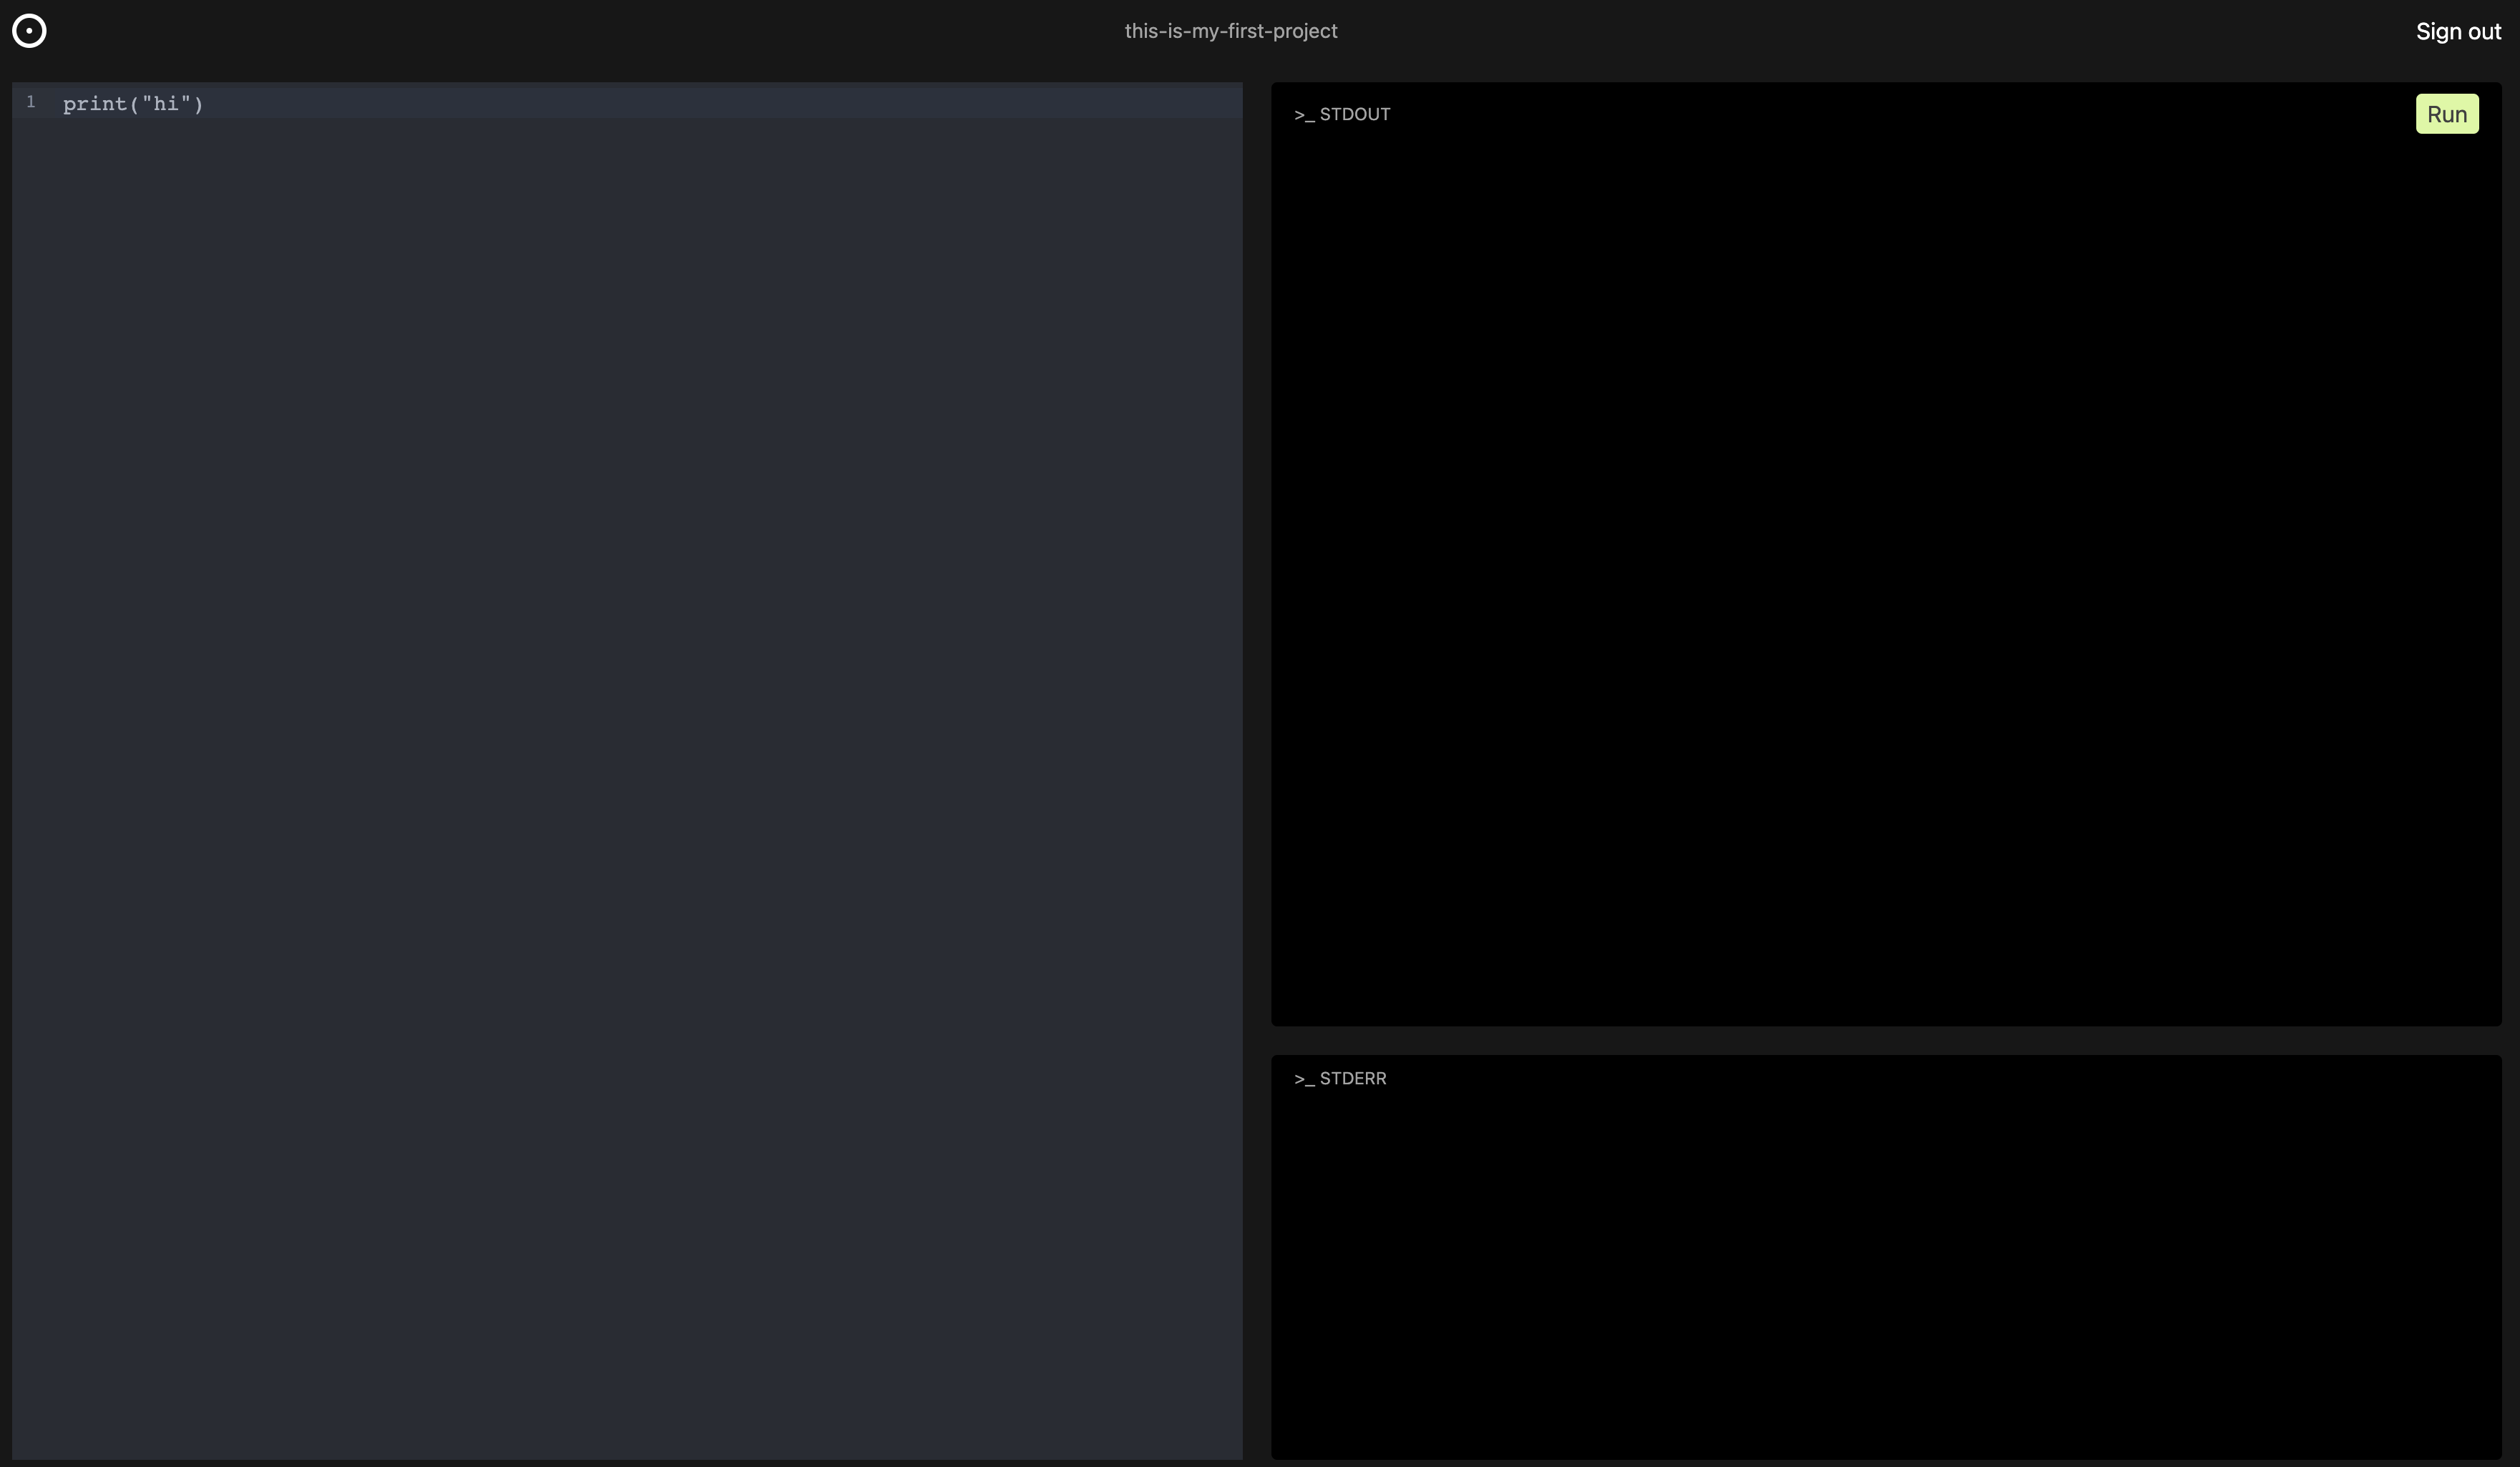
\includegraphics[width=\textwidth]{./3-Design/editor.png}
        \caption{صفحه ادیت کد}
        \label{fig:editor}
    \end{subfigure}

    \caption{طرح برخی از صفحه ها}
\end{figure}

در شکل بالا میتوانید نمونه ای از صفحه های پیاده سازی شده در این پروژه را مشاهده کنید.


\begin{figure}[h]
    \centering
    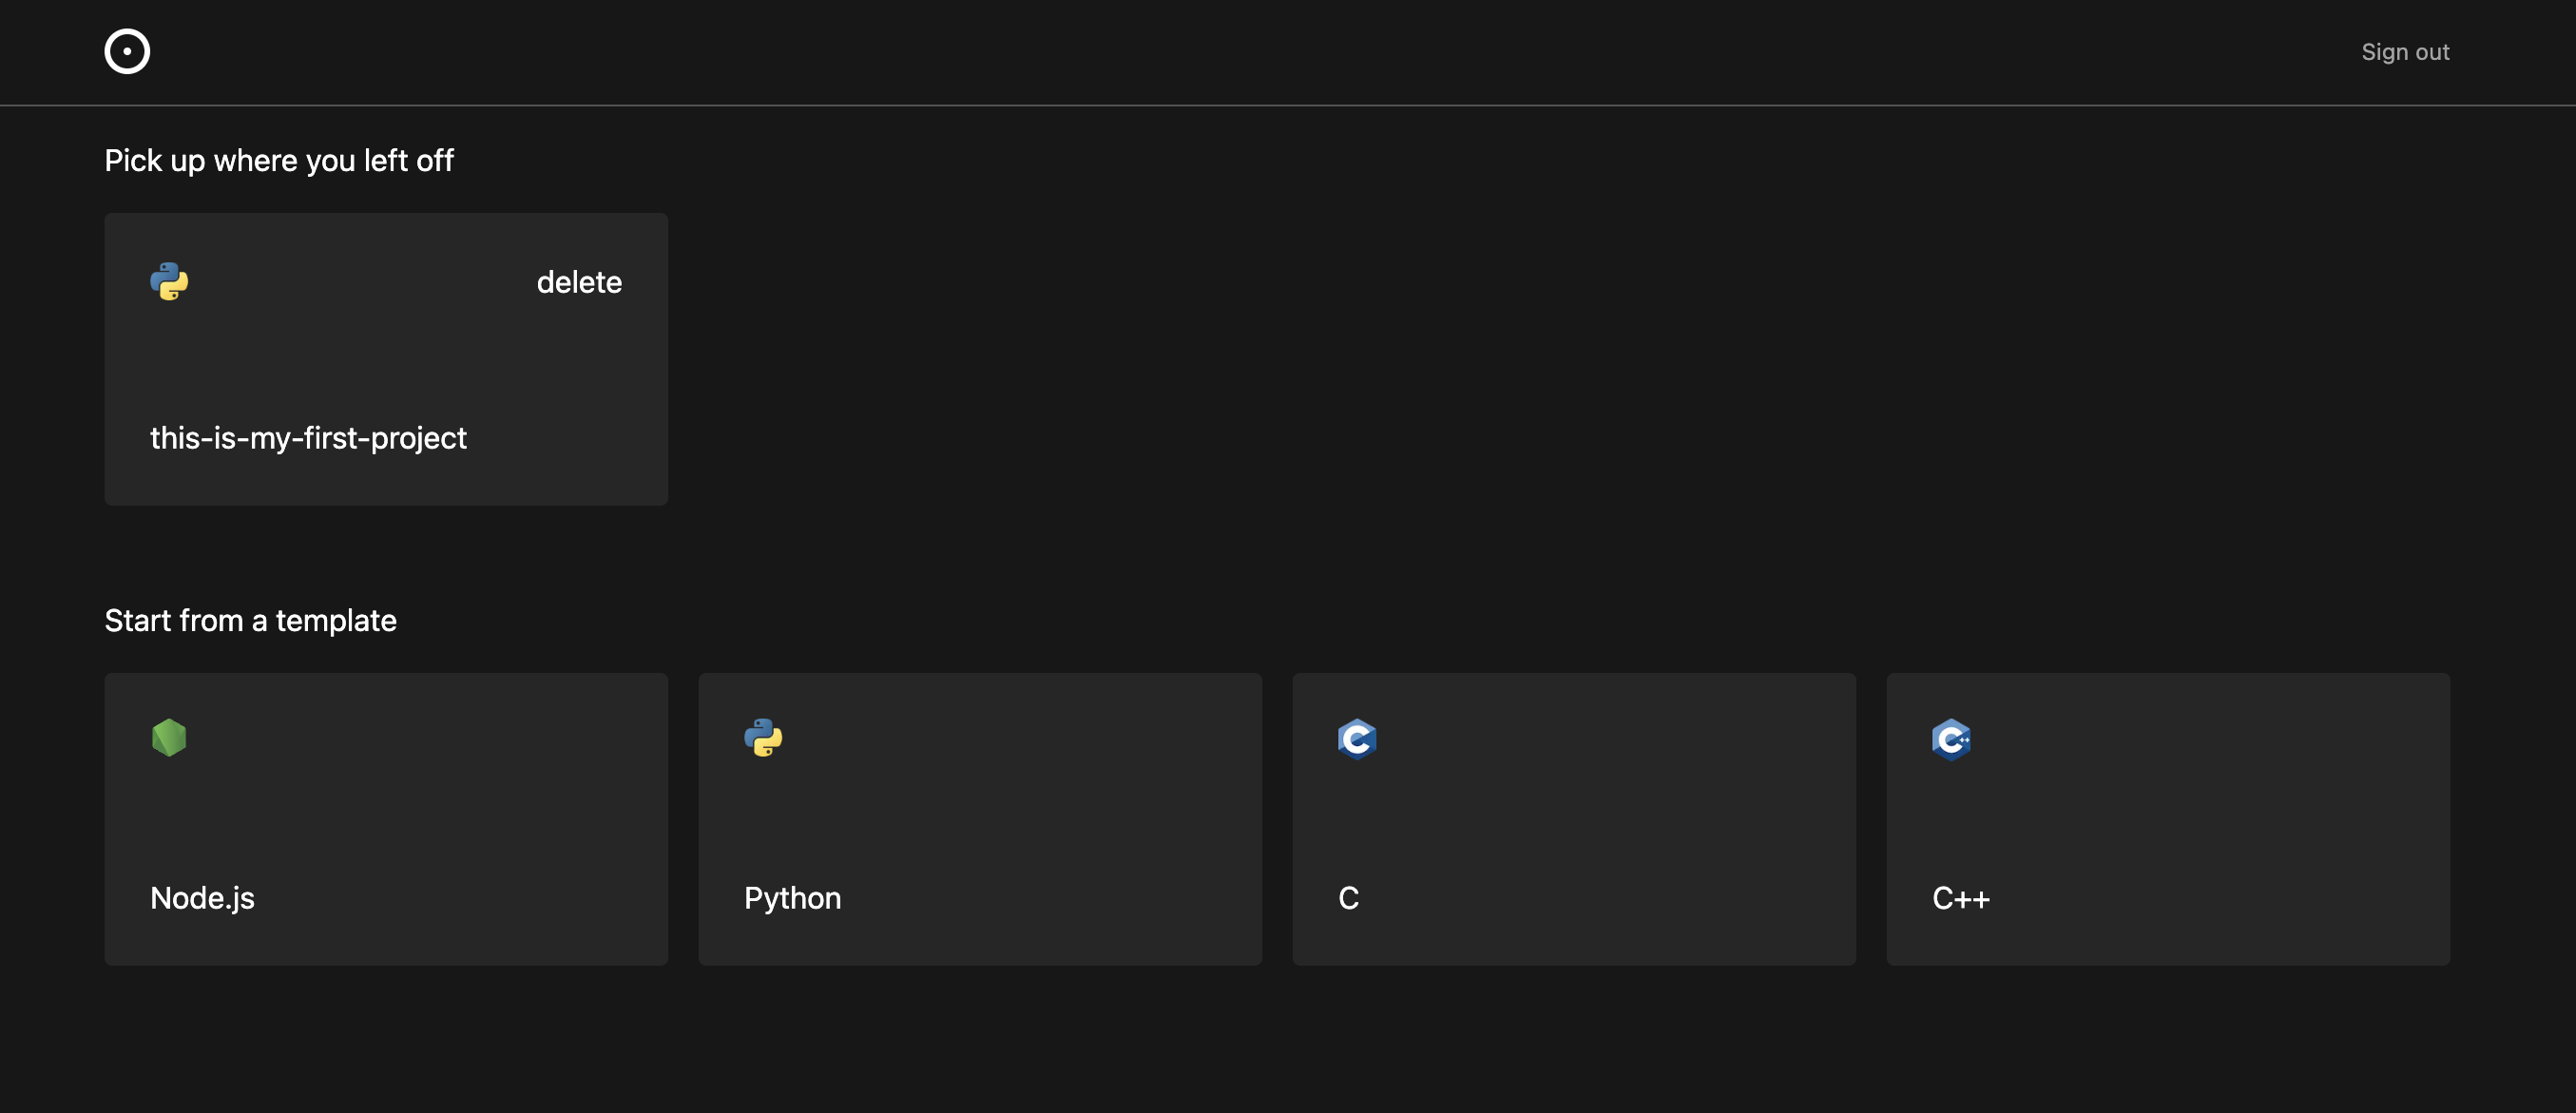
\includegraphics[width=1\textwidth]{./3-Design/projects.png}
    \caption{لیست پروژه ها}
    \label{fig:projects}
\end{figure}

پس ثبت نام و ورود به سایت شما با صفحه داشبورد مواجه می‌شوید. در این صفحه می‌توانید به ادامه ویرایش پروژه قبلی خود بپردازید یا توسط قالب های از پیش تعیین شده پروژه جدیدی شروع کنید.
اضافه کردن اکثر زبان های برنامه نویسی ممکن است ولی در حال حاضر از Python، Node.js، C و C++ پشتیبانی می‌شود.
